\documentclass[11pt]{article}

\usepackage[margin=1.1in]{geometry}
\usepackage{graphicx}
\usepackage{booktabs}
\usepackage{amsmath}
\usepackage{microtype}
\usepackage[hidelinks]{hyperref}
\usepackage{caption}
\captionsetup{font=small, labelfont=bf, width=0.92\textwidth}
\graphicspath{{../}}

\title{\textbf{What the Theory Never States:\\
Preregistered Simulations of REBUS and ALBUS}}
\author{Joshua Rogers\\ \small Independent researcher \\ \small \texttt{josh@envitae.io}}
\date{August 2026 \\ \small Preprint. Comments welcome.}

\begin{document}
\maketitle

\begin{abstract}
\noindent REBUS holds that psychedelics reduce the precision of high-level priors,
permitting belief revision that rigid priors prevent. ALBUS replies that at low doses
beliefs are instead strengthened (SEBUS), with relaxation appearing only at higher
doses. Neither account has published equations or code. We built the minimal Bayesian
agent both theories describe, preregistered the mapping from each paper's stated claims
to model parameters (committed to a git history before any code ran, for every arm),
and swept dose against evidence quality across billions of simulated agents. Three
findings. First, REBUS as literally stated produces no lasting change at all: dose
transforms the acute state, and the effect evaporates when precision returns to
baseline. The failure is structural rather than numerical, so something must make
revision stick, and that something is not in the theory. Second, adding a consolidation
process, it acts as a gate: below a threshold, lasting insight is exactly zero at every
dose, and above it dose scales the yield. But four defensible parameterizations of what
consolidation operates on disagree about whether the drug matters at all (under one,
the best available outcome occurs at dose zero), whether integration can be made safe,
and whether entrenched beliefs are treatable. The gate also passes false beliefs,
though in every mechanism tested false insight requires more consolidation than true
insight, so a safe integration window exists whose width depends on which mechanism is
right. Third, SEBUS never emerges from precision mechanics: passive relaxation,
epistemic action under a correct model, and miscalibrated self-knowledge all fail to
produce it. It appears only when the diagnostic test carries a cost. Strengthening is
avoidance, and the mediating variable identifies what the drug does: prior relaxation
raises the epistemic value of an avoided test until it is worth running. Above a cost
ceiling, no dose helps. The general lesson is methodological: implementing a theory's
functional claim forces an assumption the theory never states, and that assumption, not
the theory, decides the result. Every disagreement above is a measurable prediction.
\end{abstract}

\section{Introduction}

REBUS, for relaxed beliefs under psychedelics, proposes that psychedelics reduce the
precision of high-level priors, permitting belief revision that rigid priors would
otherwise prevent \cite{carhart2019}. ALBUS, for altered beliefs under psychedelics,
proposes that at low to moderate 5-HT2A agonism beliefs are instead strengthened, a
regime its authors call SEBUS, with REBUS-style relaxation appearing only at higher
doses \cite{safron2025}. The two theories therefore make opposite-signed predictions
at low doses. Two further published claims complete the space this paper works in:
relaxation can install false beliefs rather than only correct ones \cite{mcgovern2024},
and whatever is revised during the acute window must persist beyond it to matter
clinically \cite{zeifman2025}.

None of these four accounts is accompanied by equations, code, or a runnable
simulation, and the gap is conceded in print by the field itself \cite{mago2026}. The
closest published precedent is a two-parameter precision-weighting model fit to
neuroimaging data \cite{rajpal2022}, which contains no dose sweep, no behavior, and no
released code. So the theories are argued about in prose, and prose is forgiving in a
way that implementations are not.

This paper reports what happened when we implemented the claims as stated. The method
is deliberately austere. The agent is the minimal Bayesian belief-updater the theories
describe, the dose enters exactly where REBUS says it enters (prior precision, and
nowhere else), and every mapping choice was preregistered: the mapping document was
committed to a git repository before the code that produced any number in this paper
existed, and each later experimental arm was declared in a written amendment and
committed before that arm was implemented. Predictions that failed are reported
alongside those that held.

The contributions:

\begin{enumerate}
  \item \textbf{REBUS as stated produces no lasting change.} If dose enters only
  through a precision that returns to baseline after the acute window, dose cannot
  appear in the terminal belief. This is visible in the algebra and confirmed
  numerically: acute insight moves from 0.68 to 0.96 across the dose range while
  insight measured after the window is flat at roughly 0.68 at every dose
  (Section~\ref{sec:passive}).

  \item \textbf{Whether the drug matters is a hidden assumption.} A consolidation
  process rescues persistence, and it acts as a gate: below a threshold, lasting
  insight is exactly zero at every dose. But four defensible parameterizations of what
  consolidation operates on disagree about whether dose affects the lasting outcome at
  all, whether integration can be made safe, and whether some beliefs are treatable.
  In all four, false insight requires more consolidation than true insight, so a safe
  integration window exists (Section~\ref{sec:robustness}).

  \item \textbf{SEBUS is avoidance, not precision.} Three precision-based mechanisms
  fail to produce belief strengthening: passive relaxation, epistemic action under a
  correct generative model, and epistemic action under miscalibrated self-knowledge.
  It appears exactly when the one diagnostic test is costly enough that the agent
  declines to run it, and the mediator shows that prior relaxation works by raising
  the epistemic value of the avoided test until it clears the cost. Above a cost
  ceiling the drug cannot help at any dose (Section~\ref{sec:acting}).

  \item \textbf{A preregistration protocol for simulation research.} Simulations of
  theory are especially vulnerable to the mapping being chosen after the fact, because
  whoever picks the mapping from prose to parameters can make either theory win. The
  git-audited declare-before-implement protocol used here is cheap and fully
  reproducible, and we recommend it (Section~\ref{sec:repro}).
\end{enumerate}

We make no claim about phenomenal experience anywhere in this paper. Everything below
is belief dynamics.

\section{Related work}
\label{sec:related}

The theoretical literature on precision accounts of psychedelic action is large; the
simulation literature is nearly empty. Rajpal and colleagues \cite{rajpal2022} fit a
two-level precision-weighted model to MEG data from psychedelic sessions, with the
drug modeled as reduced prior precision. It is the formulation REBUS is stated in and
the belief update used here matches its two-parameter structure, but it involves no
action, no dose-response sweep, and its code was not released. Sandved-Smith and
colleagues \cite{sandved2021} built deep parametric active inference models of
meta-awareness with precision modulation, applied to meditation rather than
psychedelics. Fisher and colleagues \cite{fisher2024} fit an active inference model to
rat behavior under psilocybin and found that the changed parameters were forgetting
rate for losses, loss aversion, and action precision rather than learning rate, which
is congenial to the present result that precision on its own carries less of the
story than expected. Powers, Mathys and Corlett \cite{powers2017} supply the strong
prior account of hallucination, the opposite pole to REBUS, with released code. One
empirical result sits awkwardly with all precision accounts and is flagged in the
limitations: a hierarchical Gaussian filter analysis of EEG found ketamine reduced
sensory precision while psilocybin showed no significant precision effect
\cite{allohverdi2025}.

ALBUS itself \cite{safron2025} contains no simulations, no code, and no equations. To
our knowledge nobody has previously swept a dose parameter through a single
implemented model and reported where SEBUS gives way to REBUS, which is the experiment
this paper runs.

\section{The model and the preregistered mapping}
\label{sec:model}

\subsection{Generative model}

A single hidden state factor, context, with $K = 6$ mutually exclusive hypotheses.
Context 0 is true: it is the hypothesis the world's evidence supports. Context 1 is
the agent's maladaptive prior conviction, the belief it arrives holding. Contexts 2
through 5 are alternative hypotheses, available but unsupported. Observations are
drawn from a categorical likelihood with reliability $r$:
\begin{equation}
p(o = j \mid \text{context} = i) = \begin{cases} r & i = j \\ (1-r)/(K-1) & i \neq j
\end{cases}
\end{equation}
$r$ is the setting: how informative the evidence arriving during the acute window is.
$r = 1/K$ is pure noise and $r = 1$ is perfectly diagnostic. The world is static.
REBUS is a claim about belief revision, not world dynamics, so transitions are the
identity.

\subsection{Belief updating}

The agent's belief after $t$ observations is the precision-weighted combination of
prior and accumulated evidence,
\begin{equation}
\log b_t(i) \;=\; \gamma \, u(i) \;+\; \lambda \sum_{\tau \le t} \log p(o_\tau \mid i),
\label{eq:update}
\end{equation}
normalized over $i$, where $u$ is a one-hot vector on the maladaptive hypothesis,
$\gamma$ is prior precision, and $\lambda$ is sensory precision. This is the
two-parameter structure of \cite{rajpal2022} and the formulation REBUS is stated in.
At baseline $\gamma_0 = 8$, which places prior odds of roughly 3000 to 1 on the
maladaptive belief.

\subsection{The dose mapping, and why it is the load-bearing choice}

Dose reduces prior precision, monotonically, and does nothing else:
\begin{equation}
\gamma(d) = \gamma_0 (1 - d), \qquad d \in [0, 1].
\label{eq:dose}
\end{equation}
This mapping deliberately contains no route to SEBUS: no level-dependence, no sign
flip, no low-dose strengthening term. That is the point of the design. ALBUS's
low-dose prediction is not built in, so if strengthening appears it has emerged from
the dynamics, and if it does not appear that is evidence that precision reduction
alone cannot produce it. The mapping was fixed in the preregistration document and
committed before any sweep ran.

Relaxation applies during an acute window of $W = 12$ observations, after which
$\gamma$ returns to $\gamma_0$. Evidence accumulated during the window persists at
the precision it was encoded with. Whether a revised belief survives the prior
snapping back is the persistence measurement of \cite{zeifman2025}.

Outcomes are classified by the terminal maximum a posteriori belief: insight
(context 0), no change (context 1), or false insight (contexts 2 through 5, the
outcome of \cite{mcgovern2024}). The preregistration fixed these definitions, seven
numbered predictions, and a falsification criterion before any code ran.

\section{REBUS as stated produces no lasting change}
\label{sec:passive}

At reliability 0.55, dose drives acute insight (measured at the end of the window)
from 0.684 to 0.963 and collapses conviction in the maladaptive belief from 0.318 to
0.012. Measured after the window, insight is flat at roughly 0.68 at every dose.

The reason is visible in Equation~\ref{eq:update}. The terminal belief is
$\mathrm{softmax}(\gamma_0 u + \lambda \, \mathrm{cum})$ where $\mathrm{cum}$ is the
accumulated log likelihood, which depends only on reliability and the random draws.
Dose enters solely through $\gamma(d)$, which applies during the window and is gone
afterwards. Dose cannot appear in the terminal belief. The acute experience is real
and it evaporates completely.

This was a preregistered prediction failure: prediction 1 expected lasting insight to
form a ridge in the dose-by-reliability plane, and there is no ridge because there is
no persistence at all. We report it as the first result rather than as a bug because
it is a statement about the theory: if the only thing the drug does is transiently
reduce prior precision, nothing lasts. Something must make the revision stick, and
that something is not in REBUS.

Adding the uncontroversial extra assumption that high doses also degrade sensory
processing (a separate arm, since it is not part of REBUS) makes dose monotonically
harmful rather than producing an interior optimum, because there is no persisting
benefit for the cost to trade against. That was prediction 5, which also failed.

\section{Consolidation: a gate, a gain, and four ways to read it}
\label{sec:robustness}

\subsection{The gate}

We then added the missing ingredient in its simplest form: a consolidation parameter
$c$, where the post-window prior is $(1-c) \cdot p_{\text{orig}} + c \cdot
b_{\text{window}}$. Table~\ref{tab:gate} shows the result. Below $c \approx 0.5$ the
lasting insight rate is exactly zero at every dose. No amount of prior relaxation
helps. Above the threshold, dose determines how much you get. Integration is
necessary, dose is not sufficient, and the two are not interchangeable.

\begin{table}[t]
\centering
\caption{Persistent insight rate by consolidation $c$ and dose $d$, reliability 0.55,
arithmetic mechanism. Below the threshold the rate is exactly zero at every dose.}
\label{tab:gate}
\begin{tabular}{lcccc}
\toprule
$c$ & $d=0.0$ & $d=0.4$ & $d=0.8$ & $d=1.0$ \\
\midrule
0.00 to 0.45 & 0.000 & 0.000 & 0.000 & 0.000 \\
0.50 & 0.090 & 0.352 & 0.480 & 0.545 \\
0.55 & 0.505 & 0.785 & 0.887 & 0.895 \\
0.80 & 0.698 & 0.863 & 0.935 & 0.965 \\
1.00 & 0.682 & 0.897 & 0.945 & 0.990 \\
\bottomrule
\end{tabular}
\end{table}

The same gate passes false beliefs. At reliability 0.30, where the evidence arriving
during the window is close to uninformative, up to roughly a quarter of agents end up
permanently holding a belief the world does not support, and they get there through
the identical mechanism that produces genuine insight
(Figure~\ref{fig:main}, panel B).

\begin{figure}[t]
\centering
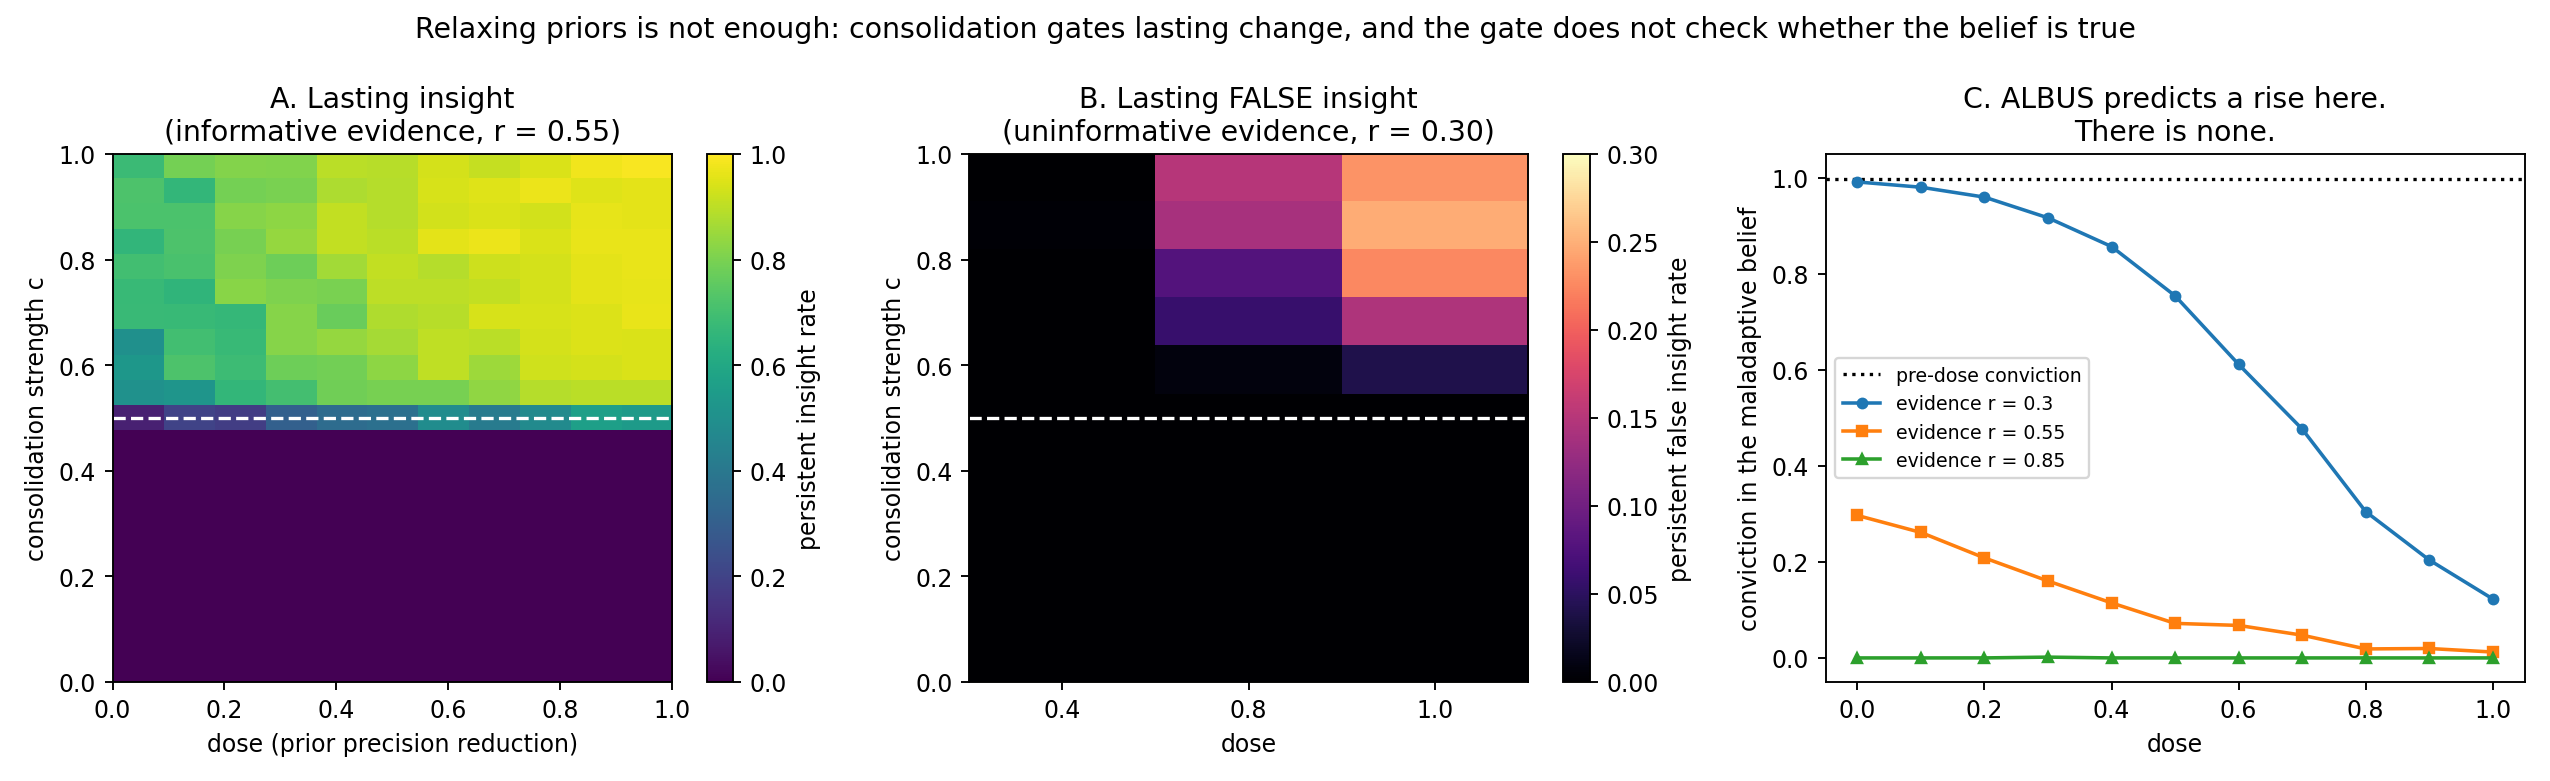
\includegraphics[width=\textwidth]{figure_main.png}
\caption{The passive agent. (A) Lasting insight by dose and consolidation under
informative evidence: a gate in $c$, a gain in dose. (B) Lasting false insight under
uninformative evidence: the same gate admits beliefs the world does not support, at
higher $c$. (C) Conviction in the maladaptive belief at window end. ALBUS predicts a
rise at low dose; conviction falls monotonically at every reliability.}
\label{fig:main}
\end{figure}

\subsection{Four parameterizations of ``the revision sticks''}

The threshold value near 0.5 is obviously an artifact of the arithmetic mixture. The
question that matters is which claims survive a change of mechanism. Four
parameterizations, each a defensible reading of what consolidation could operate on,
were declared before implementation. With $u$ the one-hot on the maladaptive
hypothesis, $p_{\text{orig}} = \mathrm{softmax}(\gamma_0 u)$, $b$ the belief at window
end, and $\mathrm{cum}$ the accumulated log likelihood:
\begin{align}
\text{P-A, arithmetic mixture:} \quad & p_{\text{after}} \propto (1-c)\,
p_{\text{orig}} + c\, b\\
\text{P-B, geometric mixture:} \quad & \log p_{\text{after}} \propto (1-c) \log
p_{\text{orig}} + c \log b\\
\text{P-C, attractor weakening:} \quad & \log p_{\text{after}} \propto \gamma_0 (1-c)\,
u + \lambda\, \mathrm{cum}\\
\text{P-D, memory trace:} \quad & \log p_{\text{after}} \propto \gamma_0 u + c\,
\lambda\, \mathrm{cum}
\end{align}
P-A and P-B act on the belief state reached during the window. P-C treats
consolidation as permanent weakening of the old attractor, and P-D as retention of a
fraction of the encoded evidence; neither looks at $b$ at all. The main grid is 8
reliabilities by 41 doses by 41 consolidation levels by 4 mechanisms by 50{,}000
trials, with observation draws shared across dose so the dose contrast is paired,
2.69 billion simulated agents in total.

\begin{table}[t]
\centering
\caption{Persistent insight at full consolidation, informative evidence. Under P-C
and P-D the spread across all 41 doses is exactly zero: dose is causally irrelevant
to the lasting outcome.}
\label{tab:mech}
\begin{tabular}{lcccc}
\toprule
dose & P-A & P-B & P-C & P-D \\
\midrule
0.00 & 0.6120 & 0.6120 & 0.9634 & 0.6120 \\
0.50 & 0.8627 & 0.8627 & 0.9634 & 0.6120 \\
1.00 & 0.9634 & 0.9634 & 0.9634 & 0.6120 \\
\midrule
spread across all doses & 0.3514 & 0.3514 & 0.0000 & 0.0000 \\
\bottomrule
\end{tabular}
\end{table}

Table~\ref{tab:mech} is the central result of this section. In the two mechanisms
where consolidation acts on the belief state reached during the window, dose changes
the lasting outcome substantially. In the two where it acts on the attractor or on
the encoded evidence, dose is causally irrelevant at every dose and every
reliability, exactly and not approximately. Note the P-C column: under the attractor
account the best available outcome is reached with no drug at all, purely by
weakening the old conviction. The therapeutic relevance of the acute experience is
not a finding of REBUS. It is a hidden assumption about what consolidation operates
on, and neither REBUS nor the persistence literature states it.

\subsection{The gate is not blind, which is better news than the alternative}

An earlier version of this work claimed, from the arithmetic mechanism alone, that no
setting of $c$ separates true from false insight. That claim was wrong in general and
is corrected here. Table~\ref{tab:window} gives the onset of each outcome as $c$
rises. In three of four mechanisms the separation is wide, and under P-D poor
evidence never produces a persistent false belief at any consolidation level, because
with uninformative evidence the old conviction simply wins rather than being
displaced by noise.

\begin{table}[t]
\centering
\caption{Onset in $c$ of each outcome at dose 0.8. False insight always requires
more consolidation than true insight.}
\label{tab:window}
\begin{tabular}{lccc}
\toprule
mechanism & true onset & false onset & separation \\
\midrule
P-A arithmetic & 0.500 & 0.600 & 0.100 \\
P-B geometric & 0.375 & 0.775 & 0.400 \\
P-C attractor & 0.175 & 0.525 & 0.350 \\
P-D memory & 0.525 & never & total \\
\bottomrule
\end{tabular}
\end{table}

The invariant that survives every mechanism, every hypothesis count $K \in \{3, 6,
10, 20\}$, and every window length in $\{4, 12, 30\}$ is: false insight always
requires more consolidation than true insight. In every cell of the structural sweep
where both onsets are defined, the false onset exceeds the true onset, with no
reversals. So the defensible claim is not that integration is indiscriminate. It is
that integration admits true beliefs at a lower threshold than false ones, so there
exists a window in which it helps without hurting, and the width of that window
depends on a mechanism nobody has pinned down. Which measurement would settle the
question is exactly the disagreement between the columns of
Table~\ref{tab:window}.

Two further mechanism-dependent disagreements are shown in
Figure~\ref{fig:robustness}. The sharpness of the consolidation threshold varies by a
factor of three across mechanisms, so the hard step in the single-mechanism result
oversold how knife-edged the transition is. And as the original conviction hardens
(entrenchment $\gamma_0$ rising from 4 to 24), the consolidation required for a 50
percent lasting insight rate barely moves under P-A but climbs steeply under the
others; under P-D, past $\gamma_0 \approx 12$, no amount of consolidation reaches 50
percent. An untreatable regime exists under one defensible mechanism and not under
another, and whether it exists in reality is an empirical question about which
mechanism is right.

\begin{figure}[t]
\centering
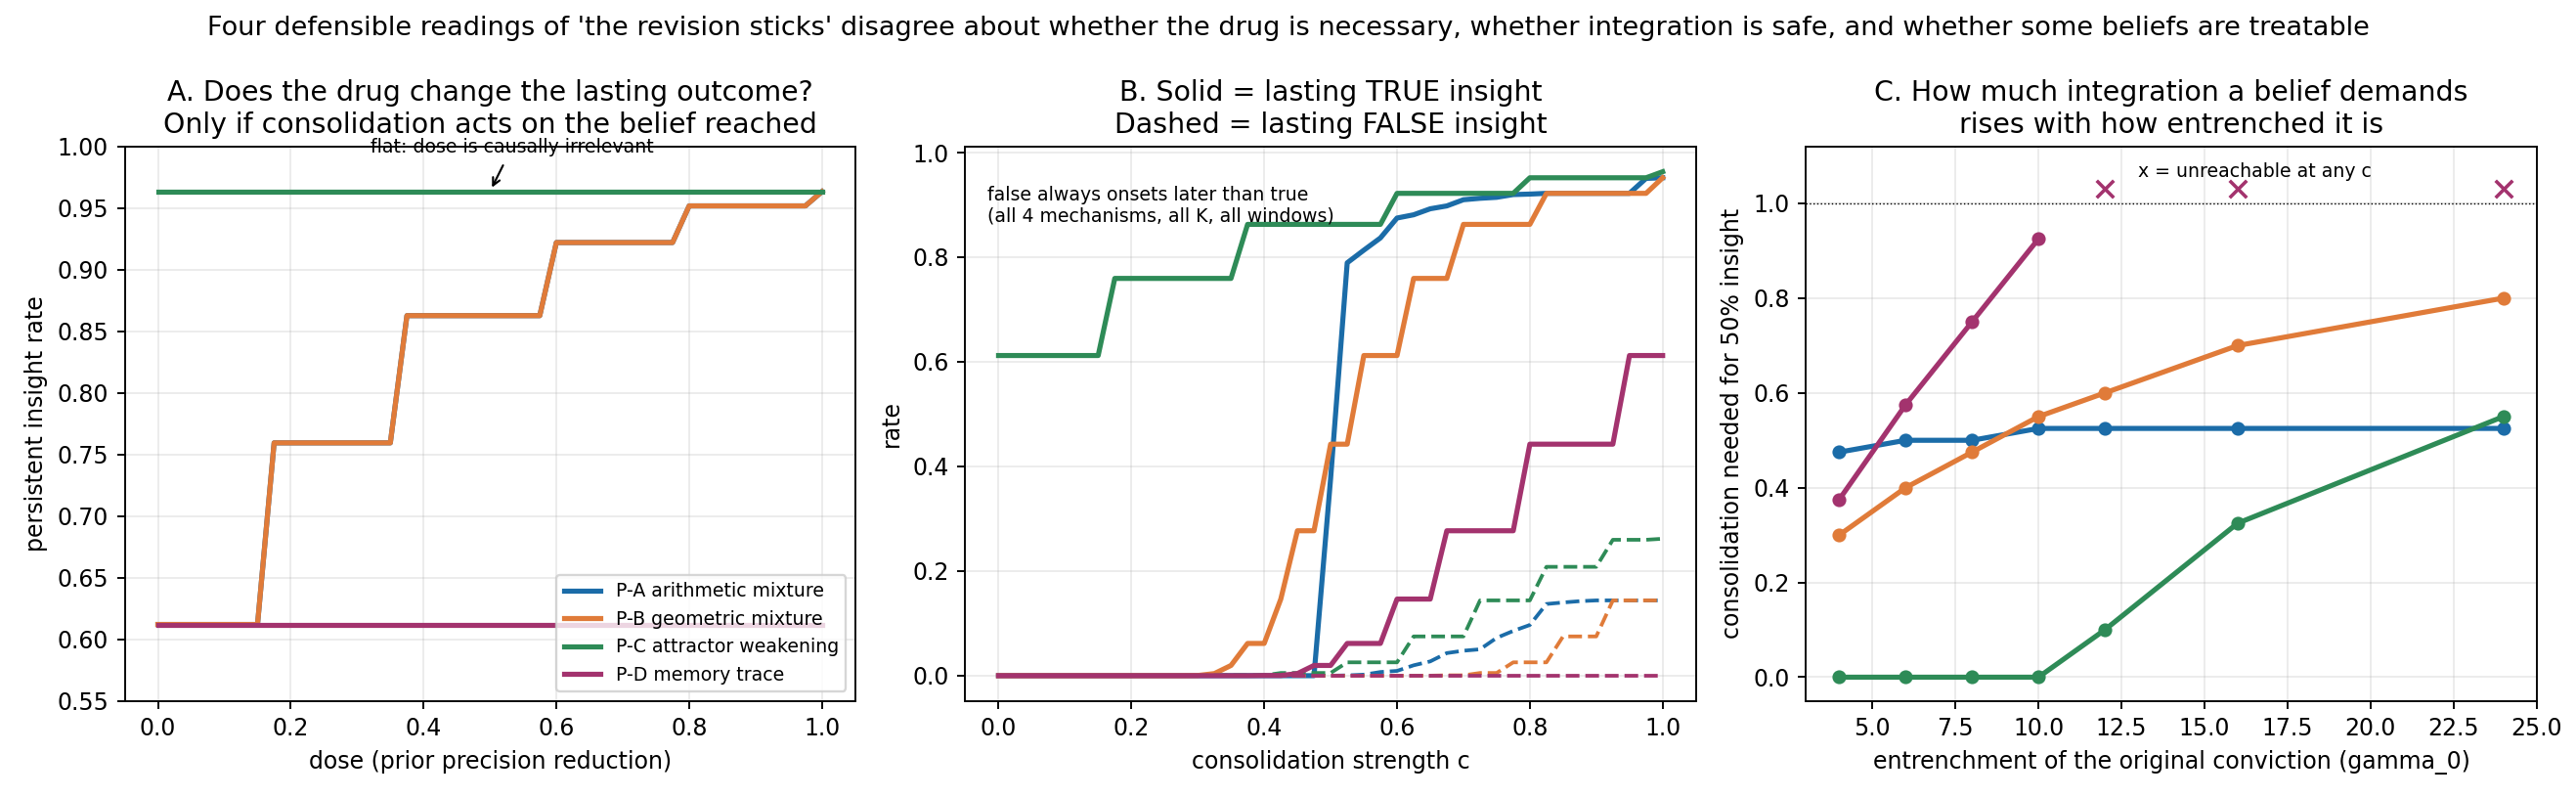
\includegraphics[width=\textwidth]{figure_robustness.png}
\caption{Four parameterizations of consolidation. (A) At $c = 0.8$, dose changes the
lasting outcome under P-A and P-B and is causally irrelevant under P-C and P-D; the
attractor mechanism reaches its ceiling with no drug at all. (B) True insight (solid)
onsets at lower $c$ than false insight (dashed) in every mechanism. (C) The
consolidation demanded for a 50 percent insight rate as entrenchment rises; crosses
mark the untreatable regime where no $c$ suffices.}
\label{fig:robustness}
\end{figure}

\section{The acting agent: where SEBUS actually lives}
\label{sec:acting}

The passive agent receives evidence rather than choosing it, and the preregistration
flagged this as the reason its SEBUS null must be read narrowly: the most plausible
route to belief strengthening is confirmation sampling, a rigid belief steering the
agent toward evidence that supports it. That mechanism cannot appear in a passive
model. The acting arms build it, each declared in a written amendment before
implementation.

\subsection{Design}

Hypotheses are not equally distinguishable. The true hypothesis (0) and the
maladaptive conviction (1) are mutually confusable: each shallow probe $j$ tests
membership in a group $G_j$, with $G_0 = G_1 = \{0, 1\}$ and $G_j = \{j\}$ for $j \ge
2$, so shallow probes can eliminate the irrelevant alternatives but can never
separate 0 from 1. One deep probe separates 0 from 1 and is uninformative about
everything else. Action is selected by softmax over the epistemic value of each probe
(the expected reduction in uncertainty under the agent's current beliefs), with no
reward term and no preference that could smuggle in a bias toward the maladaptive
hypothesis. Dose enters exactly as before, through Equation~\ref{eq:dose}. Runs
total roughly $10^8$ agent trajectories at 14 decision steps each.

\subsection{Three precision mechanisms fail for the same reason}

\begin{table}[t]
\centering
\caption{The arc of the acting arms. Each row was declared, with numbered
predictions, before its code was written.}
\label{tab:arc}
\begin{tabular}{llll}
\toprule
\# & mechanism & SEBUS? & preregistered as \\
\midrule
1 & passive precision reduction & no & prediction 3, confirmed \\
2 & epistemic action, correct model & no & prediction 13, failed \\
3 & epistemic action, miscalibrated self-knowledge & no & prediction 18, failed \\
4 & epistemic action with a costly diagnostic test & yes & prediction 21, confirmed \\
\bottomrule
\end{tabular}
\end{table}

We expected the confusability structure alone to produce confirmation sampling
(prediction 13). It does not. A Bayesian agent with a correct generative model prices
the deep probe according to how much 0-versus-1 uncertainty it actually has, runs it
14 to 25 percent of the time, and two or three uses carry enough evidence to
overwhelm the maladaptive belief. Neither rigidity nor the structure stops it. The
structure is not inert: it retards revision by a factor of six (conviction 0.368
against 0.057 in a separable control). It just never reverses it.

Miscalibrated self-knowledge, in which the agent's internal model says the shallow
probes are fully diagnostic when they are not, also fails (prediction 18). It does
real damage, cutting accuracy from 0.654 to 0.416, but only one cell in the entire
grid rose above baseline, at dose zero, by 0.0067, which is not a dose effect. The
diagnosis across both failures is the same: in every precision-based arm a genuinely
diagnostic test exists, the agent's epistemic drive prices it correctly, and an agent
with a working epistemic appetite finds the question that matters. The missing
ingredient is not precision or calibration. It is whether the agent is willing to run
the test at all.

\subsection{A costly test produces SEBUS, and dose opens it}

Real diagnostic tests are effortful or aversive; confronting the belief that
organizes your self-model is the expensive thing, which is what avoidance means
clinically. Giving the deep probe a cost, subtracted from its epistemic value before
action selection and swept from zero upward with nothing else changed, produces the
strengthening regime (Table~\ref{tab:cost}). There is a threshold between cost 0.2
and 0.3, and above it the agent ends the window more convinced of the untested belief
than it began.

\begin{table}[t]
\centering
\caption{Conviction at window end against a pre-dose baseline of 0.8007,
entrenchment 3.0. SEBUS appears above a cost threshold, and the SEBUS-to-REBUS
crossover moves to higher dose as cost rises.}
\label{tab:cost}
\begin{tabular}{lccc}
\toprule
test cost & peak conviction & delta vs baseline & dose range showing SEBUS \\
\midrule
0.00 & 0.3676 & $-0.4331$ & none \\
0.10 & 0.6034 & $-0.1973$ & none \\
0.20 & 0.7948 & $-0.0059$ & none \\
0.30 & 0.8897 & $+0.0891$ & 0.00 to 0.23 \\
0.50 & 0.9357 & $+0.1351$ & 0.00 to 0.42 \\
0.80 & 0.9442 & $+0.1435$ & 0.00 to 0.50 \\
1.20 & 0.9455 & $+0.1448$ & 0.00 to 0.50 \\
\bottomrule
\end{tabular}
\end{table}

So SEBUS is not a precision phenomenon. It is an avoidance phenomenon. Belief
strengthening requires that the agent was already declining to run the test that
would disconfirm the belief, which is why three precision-based mechanisms could not
produce it.

The mediator makes the account mechanistic (Figure~\ref{fig:acting}, panel B). With
no cost, deep-probe usage is flat and slightly falling in dose. With a cost, usage
rises with dose: relaxing the prior raises the agent's uncertainty about the
distinction that matters, which raises the epistemic value of the test, which pushes
it back above the cost. Prior relaxation causes the agent to face a test it was
avoiding. That is a mechanistic account of what the drug does, and neither REBUS nor
ALBUS states it. At cost 1.2 usage is 0.000 at every dose: above a cost ceiling the
drug cannot help at all, because no amount of prior relaxation makes the test worth
running.

\begin{figure}[t]
\centering
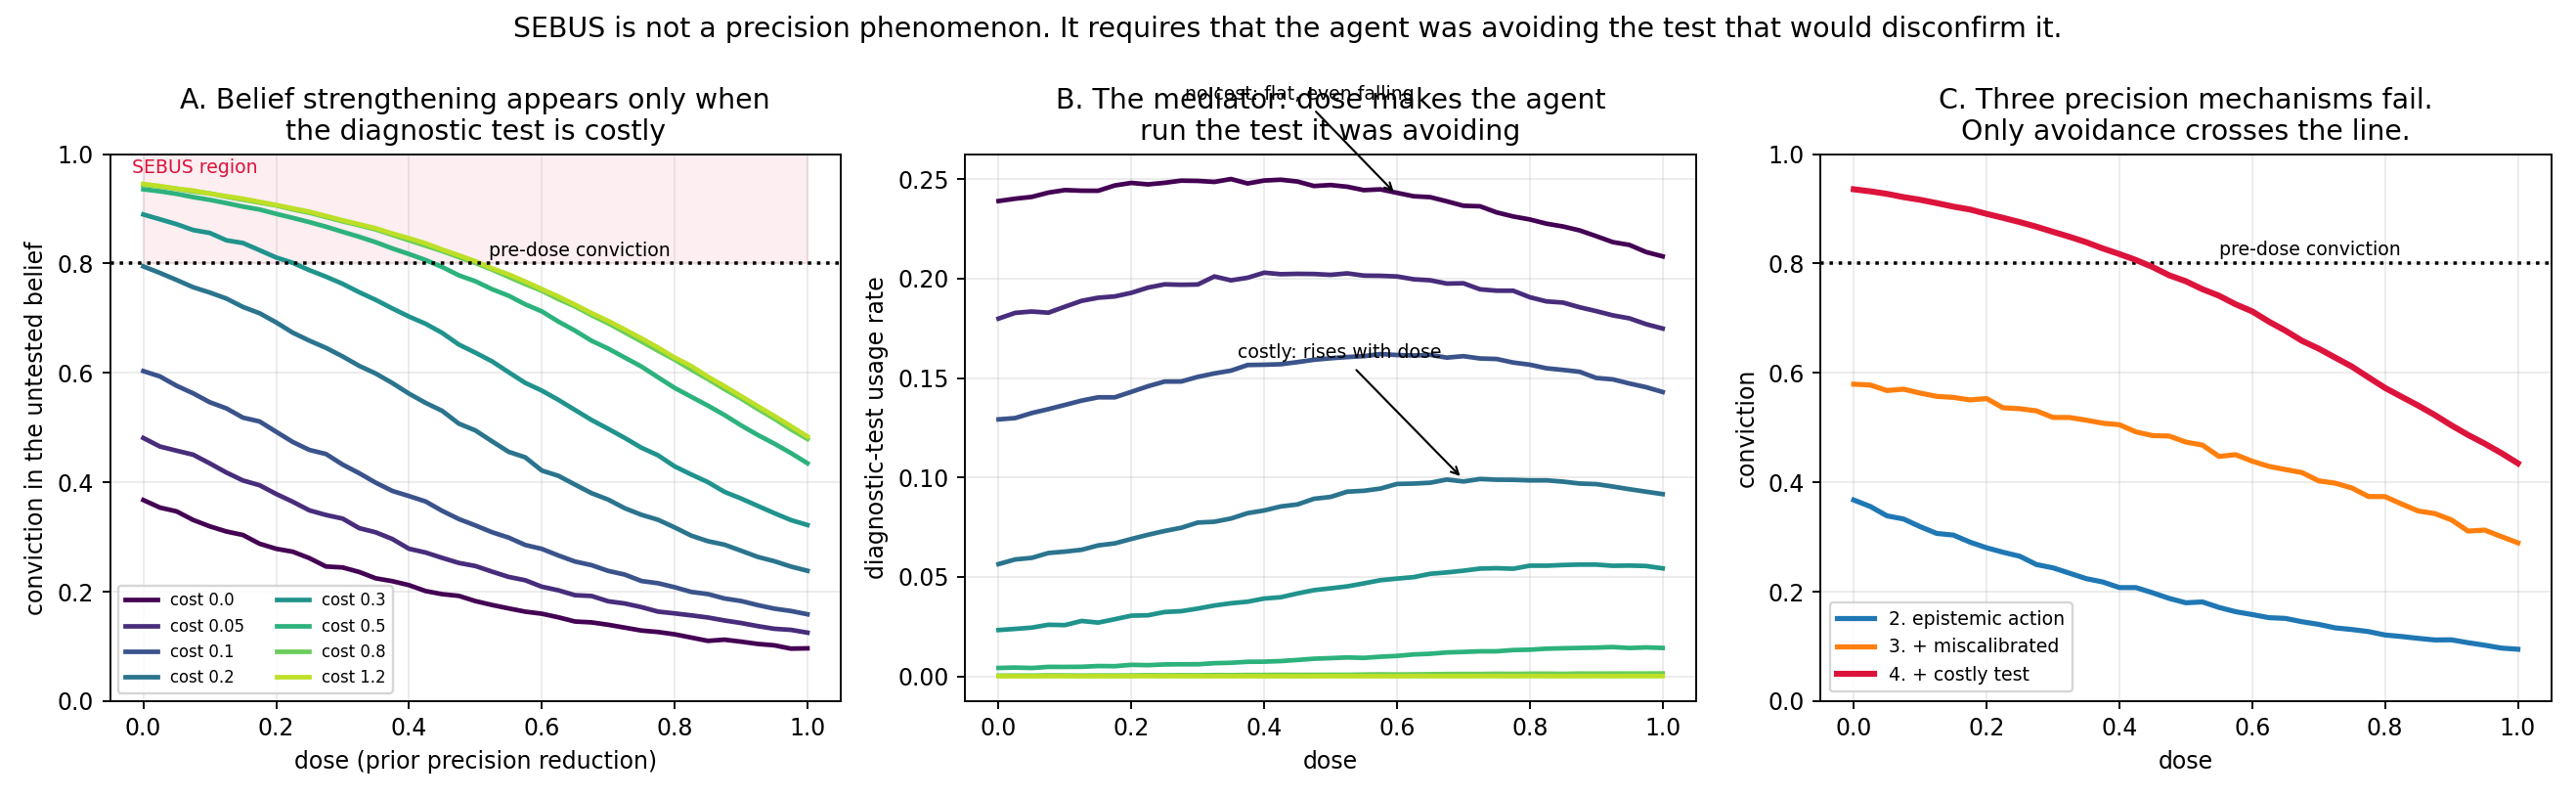
\includegraphics[width=\textwidth]{figure_acting.png}
\caption{The acting agent. (A) Conviction in the untested belief by dose, one curve
per test cost; the shaded region marks conviction above the pre-dose baseline. (B)
Diagnostic-test usage: flat in dose when the test is free, rising with dose when it
is costly. (C) The four-mechanism summary: only the costly-test mechanism crosses the
baseline.}
\label{fig:acting}
\end{figure}

One preregistered expectation was half right and the miss is informative. The
SEBUS-to-REBUS crossover exists and moves to higher dose as cost rises, from dose
0.23 at cost 0.3 to 0.50 at cost 0.8, which is ALBUS's structure: a low-dose regime
of strengthened belief giving way to a high-dose regime of relaxation. But peak
conviction is always at dose zero, so the curve within the SEBUS region is
flat-to-declining rather than rising. The drug never adds strengthening. It fails to
remove pre-existing strengthening until the dose is high enough. ALBUS as usually
read implies the drug actively strengthens beliefs at low doses, and nothing here
does that.

\section{What to claim, and what not to}
\label{sec:claims}

\textbf{Claim.} REBUS as stated is incomplete: without a consolidation process
nothing lasts, and which of four defensible consolidation mechanisms is right decides
whether the drug matters at all, whether integration can be made safe, and whether
some beliefs are treatable. SEBUS requires avoidance of a diagnostic test, not
altered precision: three precision-based mechanisms fail to produce it and one
avoidance-based mechanism does. The therapeutic action of prior relaxation, in this
model family, is to make an avoided test worth running, and above a cost ceiling that
mechanism is unavailable.

\textbf{Do not claim} that REBUS or ALBUS is wrong. REBUS's core within-window claim
behaves exactly as stated; what is missing is everything after the window. ALBUS's
low-dose prediction has no route through precision and needs an avoidance term, and
that term is absent from the paper; but the crossover structure the costly-test
mechanism produces is recognizably the structure ALBUS describes. Both theories are
underdetermined rather than refuted, and every point of underdetermination identified
here is a measurable prediction: which quantity consolidation tracks, whether a
dose-zero arm with integration support matches a dosed arm, whether strengthening
covaries with avoidance rather than with dose.

\section{Limitations}
\label{sec:limitations}

\begin{enumerate}
  \item \textbf{Free parameters.} The consolidation level $c$ and the test cost are
  calibrated to no clinical quantity. Every threshold reported here is an ordinal
  claim (a threshold exists, a ceiling exists, false onset exceeds true onset), not a
  number to quote.
  \item \textbf{The world is static and small.} Six hypotheses, one maladaptive
  belief, one diagnostic test, identity transitions. This models belief revision,
  not a changing environment, and the confusability structure is hand-built.
  \item \textbf{The cost is imposed, not derived.} Avoidance is implemented as a
  fixed price on one probe. A fuller model would derive avoidance from the agent's
  own preferences, for instance aversion to expected belief change in a
  self-relevant hypothesis.
  \item \textbf{Belief dynamics only.} Nothing here bears on phenomenal experience,
  neuropharmacology, or any subjective quality of the acute state. The model treats
  the window entirely as an evidence-and-precision episode.
  \item \textbf{One empirical result sits awkwardly with all of this.} A
  hierarchical Gaussian filter analysis of EEG found ketamine reduced sensory
  precision while psilocybin showed no significant precision effect
  \cite{allohverdi2025}. If psilocybin does not measurably move precision, every
  precision-mapped simulation, including this one, is modeling a mechanism whose
  empirical footing is unsettled.
  \item \textbf{Failed predictions are part of the record.} Predictions 1 and 5
  (ridge and interior optimum) failed in the passive arm, and predictions 13, 16 and
  18 (SEBUS from confusability alone, mediation without cost, SEBUS from
  miscalibration) failed in the acting arms. The headline results of this paper are
  downstream of those failures, which is what the preregistration protocol is for.
\end{enumerate}

\section{Reproducibility}
\label{sec:repro}

The repository contains the preregistration, five amendments, all code, all result
files, and the git history that orders them. The mapping was committed at
\texttt{8109e7f} before any sweep ran; the consolidation arm was declared at
\texttt{860c369}, the four parameterizations at \texttt{d003810}, the acting agent at
\texttt{ca4622e}, miscalibration at \texttt{b9a5d47}, and the costly test at
\texttt{daef447}, each before the corresponding code existed. Simulations are
pure NumPy with fixed seeds; the passive grids run in minutes on a laptop and the
full robustness grid (2.69 billion agents) in under an hour. Total API spend for
everything in this paper: \$0.

\begin{thebibliography}{99}

\bibitem{carhart2019} R.~L. Carhart-Harris and K.~J. Friston. REBUS and the
anarchic brain: Toward a unified model of the brain action of psychedelics.
\emph{Pharmacological Reviews}, 71(3):316-344, 2019.

\bibitem{safron2025} A.~Safron, A.~Juliani, N.~Reggente, V.~Klimaj, and
M.~Johnson. On the varieties of conscious experiences: Altered beliefs under
psychedelics (ALBUS). \emph{Neuroscience of Consciousness}, 2025(1):niae038, 2025.

\bibitem{mcgovern2024} H.~T. McGovern, H.~J. Grimmer, M.~K. Doss, B.~T.
Hutchinson, C.~Timmermann, A.~Lyon, P.~R. Corlett, and R.~E. Laukkonen. An
integrated theory of false insights and beliefs under psychedelics.
\emph{Communications Psychology}, 2:69, 2024.

\bibitem{zeifman2025} R.~J. Zeifman et al. Relaxed beliefs under psychedelics
(REBAS): Evidence for lasting belief change after psychedelic experiences.
\emph{Scientific Reports}, 15:3651, 2025. [Title to be verified against the
published record before submission.]

\bibitem{mago2026} J.~Mago et al. Computational approaches to psychedelic
action: Promises and limits. \emph{Neuroscience of Consciousness}, 2026. [Title
to be verified against the published record before submission.]

\bibitem{rajpal2022} H.~Rajpal, P.~A.~M. Mediano, F.~E. Rosas, et al.
Psychedelics and schizophrenia: Distinct alterations to Bayesian inference.
\emph{NeuroImage}, 263:119624, 2022.

\bibitem{sandved2021} L.~Sandved-Smith, C.~Hesp, J.~Mattout, K.~Friston,
A.~Lutz, and M.~J.~D. Ramstead. Towards a computational phenomenology of mental
action: Modelling meta-awareness and attentional control with deep parametric
active inference. \emph{Neuroscience of Consciousness}, 2021(1):niab018, 2021.

\bibitem{fisher2024} V.~Fisher et al. Computational modelling of reward
learning in rats under psilocybin. \emph{Translational Psychiatry}, 14:394,
2024. Code and data: OSF, DOI 10.17605/OSF.IO/EU8KH. [Title to be verified
against the published record before submission.]

\bibitem{powers2017} A.~R. Powers, C.~Mathys, and P.~R. Corlett.
Pavlovian conditioning-induced hallucinations result from overweighting of
perceptual priors. \emph{Science}, 357(6351):596-600, 2017.

\bibitem{allohverdi2025} T.~Allohverdi et al. Hierarchical Gaussian filter
analysis of EEG under ketamine and psilocybin. \emph{bioRxiv}, 2025. [Title and
author list to be verified against the published record before submission.]

\end{thebibliography}

\end{document}
